% !TeX program = lualatex
% QuickSyn session report for 20261012_005651_FSW-0020_00000007
% Written by quicksyn_veusz_export_v0_0_6.py 0.0.6 (GPL-3.0-or-later). Compile with LuaLaTeX, twice:
%     lualatex quicksyn_session_report.tex
\documentclass[11pt]{article}
\usepackage[letterpaper,margin=2cm]{geometry}
\usepackage{fontspec}
\usepackage{amsmath}
\usepackage{booktabs}
\usepackage{array}
\usepackage{graphicx}
\usepackage{xcolor}
\usepackage{fancyhdr}
\usepackage[bookmarks=true,bookmarksnumbered=true,bookmarksopen=true,bookmarksopenlevel=2,hidelinks]{hyperref}
\usepackage{bookmark}
\hypersetup{
  pdftitle={QuickSyn session report: 20261012\_005651\_FSW-0020\_00000007},
  pdfauthor={QuickSyn Session Reduction and Veusz Export 0.0.6},
  pdfsubject={QuickSyn telemetry session: statistics and plots},
  pdfkeywords={QuickSyn, SCPI, telemetry, Allan deviation, Veusz},
  pdfcreator={LuaLaTeX},
  pdfpagemode=UseOutlines, pdfstartview=FitH}
\setlength{\parindent}{0pt}
\setlength{\parskip}{0.5\baselineskip}
\setlength{\headheight}{14pt}
\pagestyle{fancy}
\fancyhf{}
\lhead{\small QuickSyn session 20261012\_005651\_FSW-0020\_00000007}
\rhead{\small\thepage}
\lfoot{\scriptsize Generated by quicksyn\_veusz\_export\_v0\_0\_6.py 0.0.6}
\title{QuickSyn session report\\[0.3em]\large 20261012\_005651\_FSW-0020\_00000007}
\author{QuickSyn Session Reduction and Veusz Export 0.0.6}
\date{Session 2026-10-12 00:56:51 UTC (UTC+0000) to 2026-10-12 00:57:31 UTC (UTC+0000)}
\begin{document}
\maketitle
\thispagestyle{fancy}
\begin{center}\fcolorbox{red}{white}{\parbox{0.9\linewidth}{\centering
\textbf{SIMULATED SESSION:} no instrument was connected; every value
below comes from the controller's built-in simulator.}}\end{center}

\pdfbookmark[1]{Contents}{contents}
\tableofcontents
\clearpage

\section{Instrument}

\begin{center}
\begin{tabular}{@{}p{0.3\linewidth}p{0.62\linewidth}@{}}
\toprule
\textbf{Field} & \textbf{Value} \\
\midrule
\texttt{*IDN?} reply & \texttt{Phase Matrix,FSW-0020,00000007,0106,300A} \\
Model & FSW-0020 \\
Option field & \texttt{00000007} \\
Software version field & \texttt{0106} (= 106) \\
Serial field & \texttt{300A} \\
Datasheet coverage & 0.5 to 20 GHz \\
Transport & SIM at 115200 baud (simulated) \\
\bottomrule
\end{tabular}
\end{center}

The \texttt{*IDN?} field order is inferred from the native Get ID order in
\cite{nicomms}; it is not specified for the SCPI form.

\section{Acquisition timing}

\begin{center}
\begin{tabular}{@{}p{0.52\linewidth}p{0.28\linewidth}l@{}}
\toprule
\textbf{Quantity} & \textbf{Value} & \textbf{Unit} \\
\midrule
Samples & 401 &  \\
Loaded from & chunks &  \\
Duration & 39.9992 & s \\
Requested sample rate & 10 & Hz \\
Achieved sample rate & 10.0002 & Hz \\
Mean sample interval & 99.9979 & ms \\
Interval standard deviation (jitter) & 2.56112 & ms \\
Interval minimum & 82.5657 & ms \\
Interval maximum & 113.767 & ms \\
Jitter relative to the period & 25611.7 & ppm \\
Device I/O latency, mean & 6.1296 & ms \\
Device I/O latency, 95th percentile & 8.9224 & ms \\
Device I/O latency, maximum & 10.424 & ms \\
\bottomrule
\end{tabular}

\emph{Timing of the telemetry stream.}
\end{center}

The sample period is the reciprocal of the requested rate $f_s$,
\begin{equation}
  \tau_0 = \frac{1}{f_s},
\end{equation}
and the achievable rate is bounded by the serial round trips each sample
costs. With $N_q$ queries per sample and a mean round-trip time $t_q$,
\begin{equation}
  f_{s,\max} = \frac{1}{N_q\,t_q}.
\end{equation}
The jitter is the standard deviation of the measured intervals,
\begin{equation}
  \sigma_{\tau_0} = \operatorname{std}\left(t_i - t_{i-1}\right),
\end{equation}
taken from the monotonic clock of the logging computer.

\section{Generated signal}

\begin{center}
\begin{tabular}{@{}p{0.52\linewidth}p{0.28\linewidth}l@{}}
\toprule
\textbf{Quantity} & \textbf{Value} & \textbf{Unit} \\
\midrule
Distinct frequencies observed & 4 &  \\
Frequency minimum & 8.250000000 & GHz \\
Frequency maximum & 19.500000000 & GHz \\
Power minimum & -3.0 & dBm \\
Power maximum & +8.0 & dBm \\
RF output on, fraction of samples & 1.000 &  \\
Samples with RF unlocked & 0 &  \\
Samples with reference unlocked & 0 &  \\
Samples with voltage error & 0 &  \\
\bottomrule
\end{tabular}

\emph{Signal state reported by the instrument.}
\end{center}

Status bits are decoded from \texttt{STAT?} with the bit map of
\cite[Table 5]{nicomms}; the lock bits are set when \emph{unlocked}.

\section{Thermal}

\begin{center}
\begin{tabular}{@{}p{0.52\linewidth}p{0.28\linewidth}l@{}}
\toprule
\textbf{Quantity} & \textbf{Value} & \textbf{Unit} \\
\midrule
Internal temperature minimum & 29.0 & \textdegree{}C \\
Internal temperature maximum & 29.5 & \textdegree{}C \\
Rise over the session & +0.5 & \textdegree{}C \\
Margin to the +75 \textdegree{}C limit & 45.5 & \textdegree{}C \\
\bottomrule
\end{tabular}

\emph{Internal temperature (DIAG:MEAS? 21).}
\end{center}

The +75\,\textdegree{}C internal limit is the caution in \cite{niguide}.

\section{Stability of the reported carrier}

The fractional frequency error of sample $i$ against the median
commanded carrier $f_c$ is
\begin{equation}
  y_i = \frac{f_i - f_c}{f_c},
\end{equation}
and the overlapping Allan deviation at averaging time $\tau = m\,\tau_0$
follows IEEE Std 1139-2008 \cite{ieee1139}:
\begin{equation}
  \sigma_y^2(\tau) = \frac{1}{2\,(N-2m+1)\,\tau^2}
  \sum_{k=1}^{N-2m+1}\left(x_{k+2m} - 2x_{k+m} + x_k\right)^2,
\end{equation}
with the phase residuals
\begin{equation}
  x_k = \tau_0 \sum_{i<k} y_i .
\end{equation}
This characterises command fidelity and the logging time base, not the
phase noise of the carrier: \texttt{FREQ?} returns the commanded setting,
not a measurement of the output. Phase noise is specified separately in
the datasheet \cite{nidatasheet} and cannot be inferred from this log.

\begin{center}
\begin{tabular}{@{}rr@{}}
\toprule
\textbf{Averaging time $\tau$ (s)} & \textbf{ADEV $\sigma_y(\tau)$} \\
\midrule
0.1 & 2.137e-02 \\
0.2 & 2.623e-02 \\
0.4 & 3.570e-02 \\
0.8 & 5.042e-02 \\
1.6 & 7.262e-02 \\
3.2 & 1.074e-01 \\
6.4 & 1.687e-01 \\
12.8 & 3.058e-01 \\
\bottomrule
\end{tabular}
\end{center}

\clearpage
\section{Plots}

Every page of \texttt{quicksyn\_session.pdf}, rendered by
Veusz \cite{veusz} from \texttt{quicksyn\_session.vszh5}, included as vector
graphics. Commanded values are drawn as black diamonds.

\subsection{Overview (all quantities)}
\begin{center}
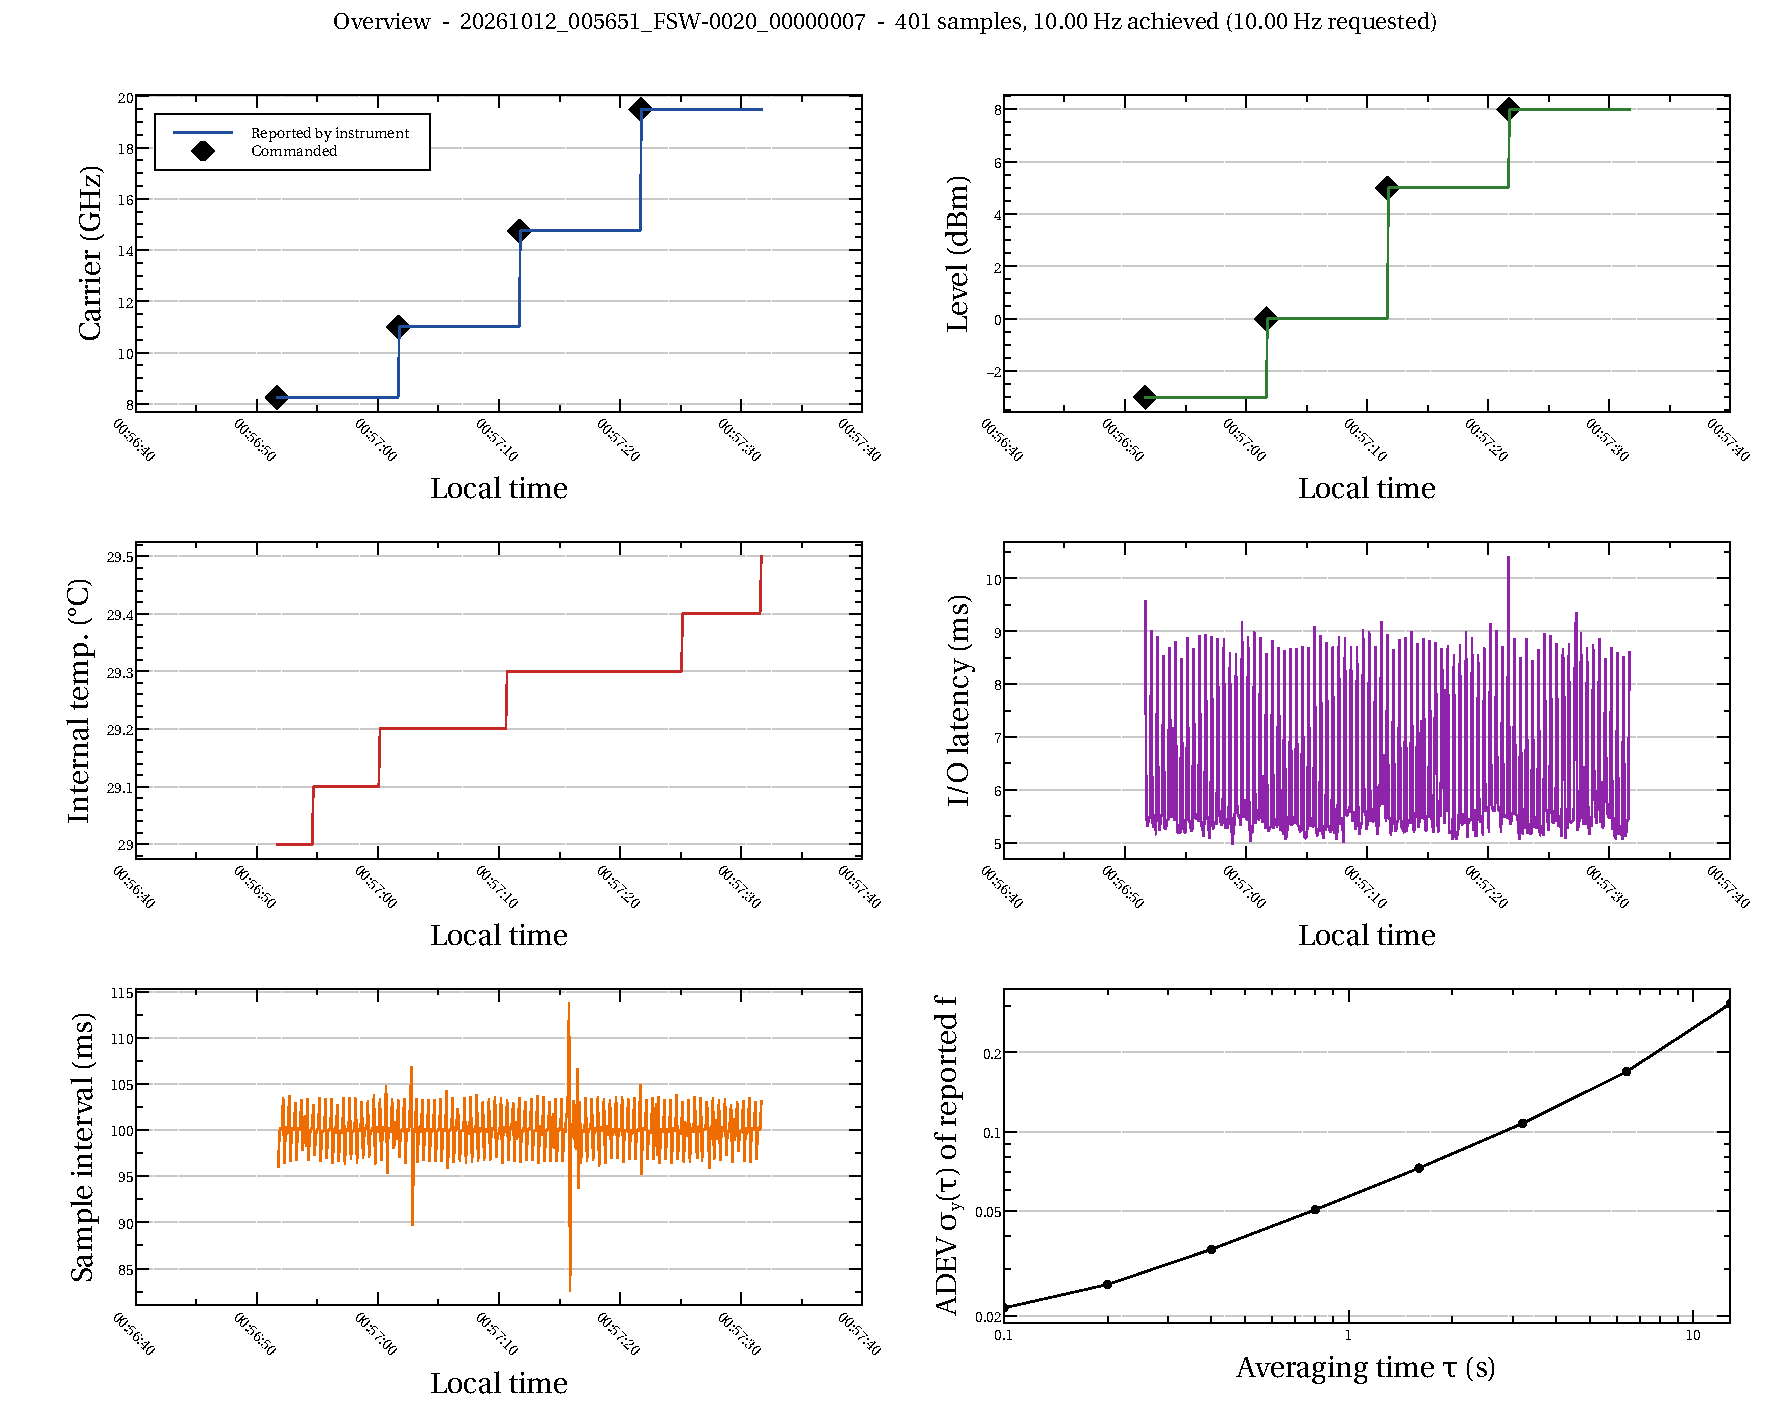
\includegraphics[page=1,width=\linewidth,height=0.78\textheight,keepaspectratio]{quicksyn_session.pdf}
\end{center}

\clearpage
\subsection{Carrier frequency}
\begin{center}
\includegraphics[page=2,width=\linewidth,height=0.40\textheight,keepaspectratio]{quicksyn_session.pdf}
\end{center}

\subsection{Output level}
\begin{center}
\includegraphics[page=3,width=\linewidth,height=0.40\textheight,keepaspectratio]{quicksyn_session.pdf}
\end{center}

\subsection{Internal temperature}
\begin{center}
\includegraphics[page=4,width=\linewidth,height=0.40\textheight,keepaspectratio]{quicksyn_session.pdf}
\end{center}

\subsection{Serial I/O latency}
\begin{center}
\includegraphics[page=5,width=\linewidth,height=0.40\textheight,keepaspectratio]{quicksyn_session.pdf}
\end{center}

\subsection{Sample interval}
\begin{center}
\includegraphics[page=6,width=\linewidth,height=0.40\textheight,keepaspectratio]{quicksyn_session.pdf}
\end{center}

\subsection{Allan deviation of the reported carrier}
\begin{center}
\includegraphics[page=7,width=\linewidth,height=0.40\textheight,keepaspectratio]{quicksyn_session.pdf}
\end{center}

\section{Files in the session folder}

\begin{itemize}
  \item \texttt{quicksyn\_session.pdf}
  \item \texttt{quicksyn\_session.vszh5}
  \item \texttt{quicksyn\_session\_p00\_page\_overview.png}
  \item \texttt{reduction\_summary.json}
  \item \texttt{reduction\_summary.md}
  \item \texttt{session.log}
  \item \texttt{session\_metadata.json}
  \item \texttt{state\_events.csv}
  \item \texttt{telemetry.csv}
  \item \texttt{telemetry\_chunk\_0000.pkl.gz}
  \item \texttt{telemetry\_reduced.npz}
  \item \texttt{transactions.csv}
  \item \texttt{quicksyn\_session\_report.tex} and \texttt{quicksyn\_session\_report.pdf} (this report)
\end{itemize}

\section{Provenance}

Statistics computed with the numpy backend in
6.6\,ms by quicksyn\_veusz\_export\_v0\_0\_6.py 0.0.6. The same numbers are
in \texttt{reduction\_summary.json} and \texttt{reduction\_summary.md}.

\phantomsection
\addcontentsline{toc}{section}{References}
\begin{thebibliography}{9}
\bibitem{nicomms} National Instruments, ``QuickSyn Microwave Synthesizers:
  Communications Specifications,'' Doc. No. 5580510-01, Santa Clara, CA, USA, 2014.
\bibitem{niguide} National Instruments, ``QuickSyn Microwave Frequency
  Synthesizer: User Guide,'' Doc. No. 5580513-01, Rev. F.
\bibitem{nidatasheet} National Instruments, ``QuickSyn Frequency Synthesizers,''
  product brochure and datasheet, Oct. 2017.
\bibitem{ieee1139} \emph{IEEE Standard Definitions of Physical Quantities for
  Fundamental Frequency and Time Metrology---Random Instabilities}, IEEE Std
  1139-2008, 2008. [Online]. Available: \url{https://ieeexplore.ieee.org/document/4797525}
\bibitem{veusz} Veusz Developers, ``Veusz---a scientific plotting package.''
  [Online]. Available: \url{https://veusz.github.io/}
\end{thebibliography}

\end{document}
